\section{Vingt-quatre étés et des feux observés}
\subsection*{Pourquoi un nouveau jeu}
Un seul mois ne permet ni saisonnalité, ni validation sur événements. Le jeu multi-annuel couvre \textbf{juin à septembre 2001--2024}, à 12 h UTC, sur la même boîte ($41\times61$ mailles) : ERA5 pour $T_{850}$, $T_{700}$ et l'humidité spécifique $q_{850}$, et les détections de feux de végétation \textbf{NASA FIRMS MODIS C6.1} (type 0, confiance $\geq30\,\%$) de neuf pays. Le point de rosée vient de la pression de vapeur exacte $e=qp/(0{,}622+0{,}378q)$ inversée par Magnus ; il n'y a plus d'humidité relative à tronquer. Seules les mailles terrestres ($\geq50\,\%$ de terre) à relief moyen $\leq1\,200$ m sont conservées : 1\,624 mailles, soit 4\,755\,072 mailles-jours.

\begin{center}
\small
\begin{tabular}{lrrr}
\toprule
Échantillon & Années & Mailles-jours & Maille-jours avec feu \\
\midrule
Apprentissage & 2001--2016 & 3\,170\,048 & 13\,206 \\
Validation & 2017--2020 & 792\,512 & 1\,856 \\
Test & 2021--2024 & 792\,512 & 1\,886 \\
\bottomrule
\end{tabular}
\end{center}
Les années entières sont séparées : aucune date n'est partagée et l'hiver sépare les saisons. Les réseaux sont entraînés sur un sous-échantillon aléatoire fixe de 200\,000 mailles-jours de l'apprentissage (dix époques, graine 100, hyperparamètres inchangés) ; les métriques portent sur toutes les mailles-jours de la validation et du test.

\begin{figure}[htbp]
\centering
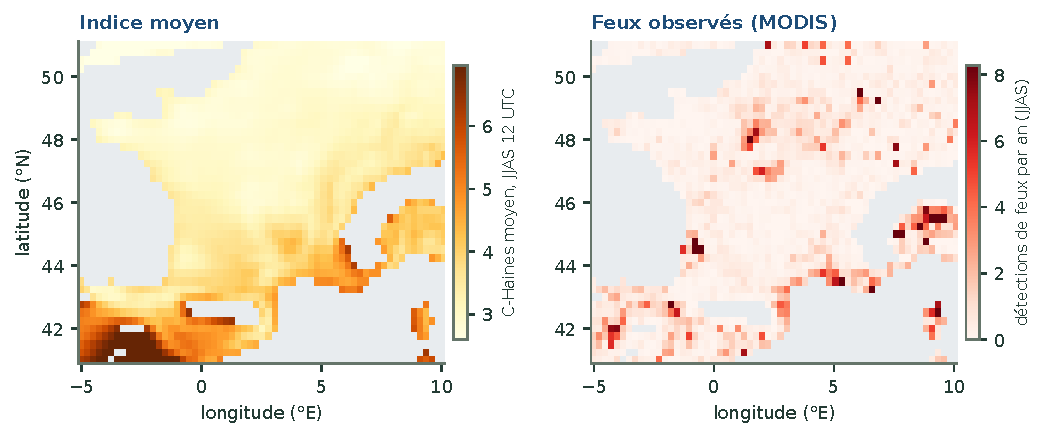
\includegraphics[width=\linewidth]{figures/fig_maps.pdf}
\caption{Indice moyen et feux observés par an sur les mailles retenues (juin à septembre, 2001--2024). L'indice est le plus élevé dans le nord de l'Espagne et par endroits sur le littoral méditerranéen ; les détections sont dispersées, avec quelques mailles de forte densité.}\label{fig:maps}
\end{figure}

\subsection*{Les modèles : un classement qui n'est pas celui de juillet}
\begin{center}
\small
\begin{tabularx}{\linewidth}{Xrrrr}
\toprule
Méthode & Wasserstein val. & Wasserstein test & Q99 généré (test) & $\Pr(H>u)$ test \\
\midrule
Référence empirique & 0,160 & 0,207 & 10,41 & 4,83\,\% \\
Référence normale & 0,255 & 0,274 & 9,81 & 2,79\,\% \\
VAE & 0,155 & 0,208 & 10,27 & 4,12\,\% \\
VAE pondéré & 0,077 & 0,123 & 10,61 & 4,68\,\% \\
GAN & 0,540 & 0,593 & 9,71 & 3,12\,\% \\
WGAN-GP & 0,227 & 0,237 & 10,72 & 4,97\,\% \\
cGAN & 0,218 & 0,266 & 10,60 & 4,71\,\% \\
\bottomrule
\end{tabularx}
\end{center}
Seuil $u=8,65$ (quantile 95\,\% de l'apprentissage) ; Q99 observé sur le test : 10,77 ; fréquence observée de dépassement sur le test : 5,13\,\%.

\textbf{Lecture.} Le \textbf{VAE pondéré} est le plus proche du test (0,123), devant la référence empirique (0,207). Le \textbf{GAN}, meilleur modèle en juillet 2023, est ici le moins bon (0,593) : le classement d'un mois ne se transpose pas. Le WGAN-GP donne le quantile 99\,\% le plus proche (10,72 contre 10,77). Tous les modèles sous-estiment la fréquence observée de dépassement, la référence empirique y compris : l'apprentissage ne reflète pas parfaitement les années 2021--2024. Une graine, dix époques et un sous-échantillon : aucun de ces écarts n'est présenté comme une supériorité établie.

\begin{figure}[htbp]
\centering
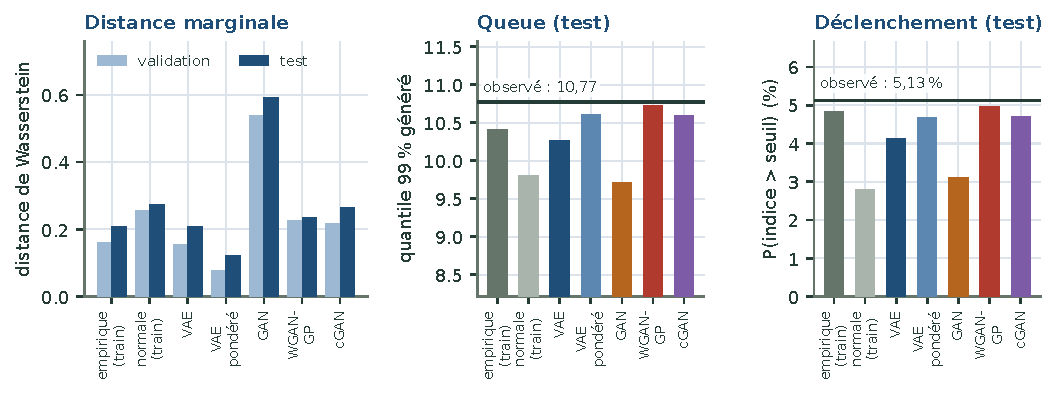
\includegraphics[width=\linewidth]{figures/fig_multi_benchmark.pdf}
\caption{Jeu multi-annuel : distance marginale (validation et test), quantile 99\,\% généré et probabilité de déclenchement face à la valeur observée sur le test (trait noir).}\label{fig:multi}
\end{figure}

\begin{figure}[htbp]
\centering
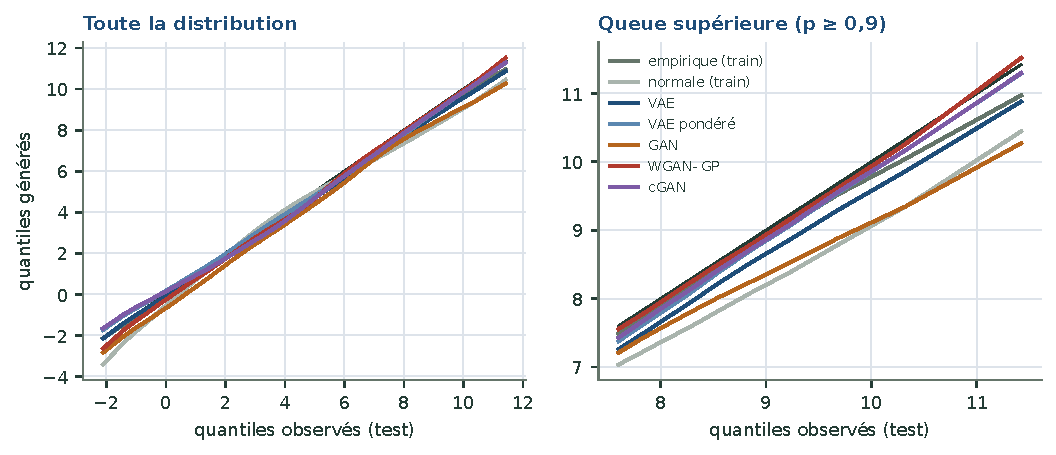
\includegraphics[width=\linewidth]{figures/fig_quantiles.pdf}
\caption{Diagramme quantile-quantile sur le test : quantiles générés contre quantiles observés (la diagonale est l'ajustement parfait). À droite, queue supérieure : le GAN et la loi normale sous-estiment la queue.}\label{fig:qq}
\end{figure}

\subsection*{L'indice est-il lié aux feux ?}
C'est la question que le mois de juillet ne pouvait pas poser. Au seuil $u$ sur le \emph{test} :
\begin{itemize}
\item la probabilité d'observer au moins un feu dans une maille-jour est de \textbf{0,57\,\%} au-dessus du seuil contre \textbf{0,22\,\%} en dessous : surcote de \textbf{$\times$2,4} ;
\item le seuil capture \textbf{12\,\%} des maille-jours avec feu, et 99,4\,\% des déclenchements n'ont aucun feu le même jour ;
\item la surcote vaut 1,4 sur l'apprentissage et 1,7 sur la validation : elle \emph{varie fortement} d'une période à l'autre.
\end{itemize}
À l'échelle de la saison, le nombre de maille-jours au-dessus du seuil et le nombre de détections de feux sont corrélés (rang de Spearman 0,57 sur 24 saisons, $p=0,004$, indicatif car les mailles sont dépendantes).

\begin{figure}[htbp]
\centering
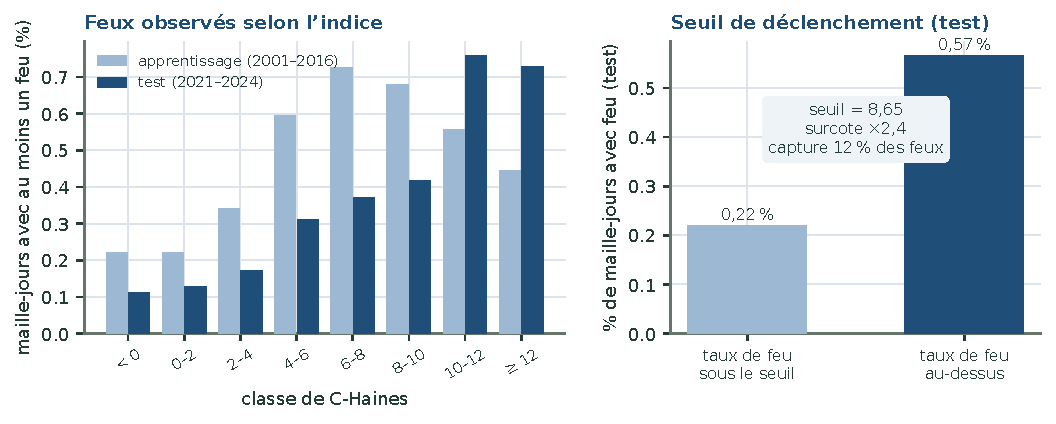
\includegraphics[width=\linewidth]{figures/fig_fire_lift.pdf}
\caption{À gauche, part de maille-jours avec au moins un feu selon la classe de C-Haines, sur l'apprentissage et le test. À droite, taux de feu sous et au-dessus du seuil sur le test, avec surcote et part des feux capturée.}\label{fig:lift}
\end{figure}

\begin{figure}[htbp]
\centering
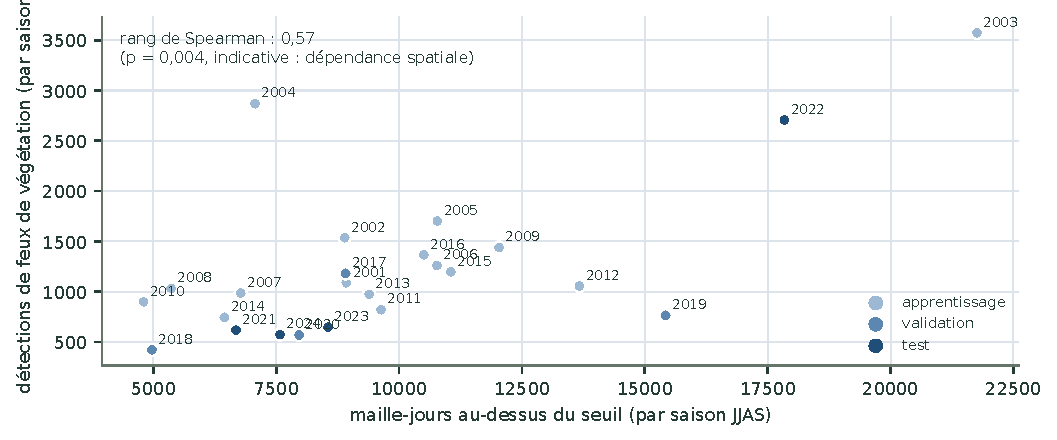
\includegraphics[width=\linewidth]{figures/fig_yearly.pdf}
\caption{Une saison par point : maille-jours au-dessus du seuil et détections de feux de végétation, avec la corrélation de rang.}\label{fig:yearly}
\end{figure}

\begin{limitbox}
\textbf{Ce que cela autorise, et ce que cela interdit.} L'indice est un signal réel mais faible à l'échelle de la maille-jour ; un contrat paramétrique sur ce seuil aurait un risque de base très élevé. FIRMS compte des détections satellitaires (brûlages agricoles compris), pas des pertes assurées ; les feux sont comptés sur la journée UTC entière, l'indice à 12 h. La part de détections retenues par le filtre passe d'environ 77\,\% (2001--2016) à environ 63\,\% (2021--2024) d'après le journal de construction ; cette dérive, non analysée, peut contribuer à la baisse du taux de feu (0,42\,\% à 0,24\,\%). Le seuil est un seuil de démonstration, non optimisé.
\end{limitbox}
